\documentclass{beamer}
\usetheme{Madrid} % My favorite!
%\usetheme{Boadilla} % Pretty neat, soft color.
%\usetheme{default}
%\usetheme{Warsaw}
%\usetheme{Bergen} % This template has nagivation on the left
%\usetheme{Frankfurt} % Similar to the default 
%with an extra region at the top.
%\usecolortheme{seahorse} % Simple and clean template
%\usetheme{Darmstadt} % not so good
% Uncomment the following line if you want %
% page numbers and using Warsaw theme%
% \setbeamertemplate{footline}[page number]
%\setbeamercovered{transparent}
\setbeamercovered{invisible}
% To remove the navigation symbols from 
% the bottom of slides%
\setbeamertemplate{navigation symbols}{} 
%
\usepackage{graphics}
\usepackage{graphicx}
\usepackage{hyperref}
\usepackage{tabularx,multirow}


%\usepackage000000..{bm}         % For typesetting bold math (not \mathbold)
\logo{
\includegraphics[height=0.6cm]{imperial.eps}}
%
\title[Cycling simulation]{Cycling simulation \\or\\ \textit{When} to break away}

\author[]{%
  Dan Demeter \and
  Alexandru Paunoiu \and
  C\'esar Prout\'e \and \\
  Julian Sutherland \and
  Robert Kruszewski
  }
\institute[Imperial College London]{  
  Imperial College London \\
  Department of Computing \\
  \vspace{1cm}
  Supervised by: Panos PARPAS\\
  
 }  

\begin{document}
%
\begin{frame}
\titlepage
\end{frame}
%

%Outline
\begin{frame}

\frametitle{Our Project}
\begin{itemize}
%% To remake good.
	\item Our Motivation
          \begin{itemize}
            \item Strategies in races can be crucial
	    \item Modelling races can lead to improved performance
          \end{itemize}
          \pause
	\vspace{0.5cm}
	\item Initial problem ( many more to come...)
          \begin{itemize}
            \item Finding optimal stategies
          \end{itemize}
%	\item Achievements \& what could we have done better 
\end{itemize}
\end{frame}


\begin{frame}
\frametitle{The solution}

\begin{itemize}
	\item Step 1: Simulation
	\item Step 2: Game theoretical model
\end{itemize}

\end{frame}


\begin{frame}
\frametitle{Step 1: Simulation}
Simulation has three parts: \\
\pause
\vspace{0.7cm}
\begin{itemize}
\item Physical model
\pause
\vspace{0.7cm}
\item Physiological model
\pause
\vspace{0.7cm}
\item Psychological model
\end{itemize}
\end{frame}

\begin{frame}
\frametitle{Physical Model}

\begin{columns}
  \begin{column}{0.6\textwidth}
    \begin{itemize}
    \item Model of the bicycle
      \vspace{0.2cm}
    \item Slipstream model (fluid dynamics)
    \end{itemize}
  \end{column}
  
  \begin{column}{0.4\textwidth}
    \begin{figure}[ht!]
      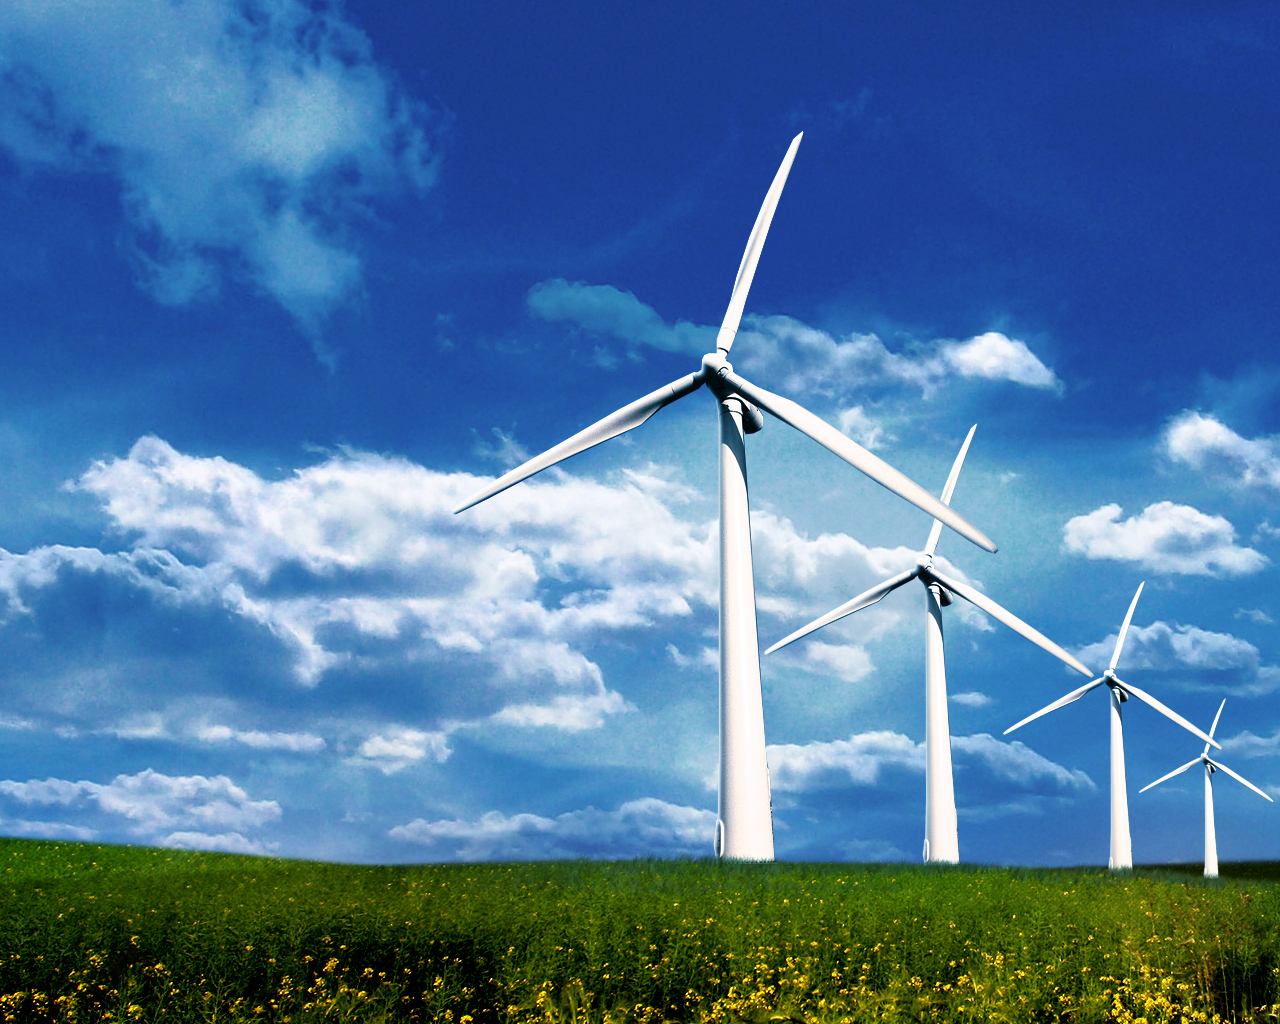
\includegraphics[scale=0.1]{physical.jpg}
    \end{figure} 
  \end{column}
\end{columns}

\end{frame}

\begin{frame}
\frametitle{Bicyle model}
The Bycicle model we used takes into account:
\begin{itemize}
\vspace{0.7cm}
\pause
\item Aerodynamic drag
\vspace{0.7cm}
\pause
\item Kinetic energy
\end{itemize}
\pause
\vspace{0.7cm}

\end{frame}

\begin{frame}
\frametitle{Assumptions}
We made some assumptions about the model:
\vspace{0.7cm}
\pause
\begin{itemize}
\item Perfectly flat race track.
\pause
\vspace{0.7cm}
\item No losses of energy due to friction.
\pause
\vspace{0.7cm}
\end{itemize}
\end{frame}

\begin{frame}
\frametitle{Slipstream model}
A Slipstream is the low pressure zone in the wake of a moving object. \newline \par
\pause
We correct for this by multiplying the aerodynamic drag by a correction factor:

$$ 0.62 - 0.0104*d_w + 0.0452*d_w^2 $$

\end{frame}

\begin{frame}
\frametitle{Correction factor}
\begin{figure}[ht!]
  \centering
    \scalebox{0.6}{% GNUPLOT: LaTeX picture with Postscript
\begingroup
  \makeatletter
  \providecommand\color[2][]{%
    \GenericError{(gnuplot) \space\space\space\@spaces}{%
      Package color not loaded in conjunction with
      terminal option `colourtext'%
    }{See the gnuplot documentation for explanation.%
    }{Either use 'blacktext' in gnuplot or load the package
      color.sty in LaTeX.}%
    \renewcommand\color[2][]{}%
  }%
  \providecommand\includegraphics[2][]{%
    \GenericError{(gnuplot) \space\space\space\@spaces}{%
      Package graphicx or graphics not loaded%
    }{See the gnuplot documentation for explanation.%
    }{The gnuplot epslatex terminal needs graphicx.sty or graphics.sty.}%
    \renewcommand\includegraphics[2][]{}%
  }%
  \providecommand\rotatebox[2]{#2}%
  \@ifundefined{ifGPcolor}{%
    \newif\ifGPcolor
    \GPcolorfalse
  }{}%
  \@ifundefined{ifGPblacktext}{%
    \newif\ifGPblacktext
    \GPblacktexttrue
  }{}%
  % define a \g@addto@macro without @ in the name:
  \let\gplgaddtomacro\g@addto@macro
  % define empty templates for all commands taking text:
  \gdef\gplbacktext{}%
  \gdef\gplfronttext{}%
  \makeatother
  \ifGPblacktext
    % no textcolor at all
    \def\colorrgb#1{}%
    \def\colorgray#1{}%
  \else
    % gray or color?
    \ifGPcolor
      \def\colorrgb#1{\color[rgb]{#1}}%
      \def\colorgray#1{\color[gray]{#1}}%
      \expandafter\def\csname LTw\endcsname{\color{white}}%
      \expandafter\def\csname LTb\endcsname{\color{black}}%
      \expandafter\def\csname LTa\endcsname{\color{black}}%
      \expandafter\def\csname LT0\endcsname{\color[rgb]{1,0,0}}%
      \expandafter\def\csname LT1\endcsname{\color[rgb]{0,1,0}}%
      \expandafter\def\csname LT2\endcsname{\color[rgb]{0,0,1}}%
      \expandafter\def\csname LT3\endcsname{\color[rgb]{1,0,1}}%
      \expandafter\def\csname LT4\endcsname{\color[rgb]{0,1,1}}%
      \expandafter\def\csname LT5\endcsname{\color[rgb]{1,1,0}}%
      \expandafter\def\csname LT6\endcsname{\color[rgb]{0,0,0}}%
      \expandafter\def\csname LT7\endcsname{\color[rgb]{1,0.3,0}}%
      \expandafter\def\csname LT8\endcsname{\color[rgb]{0.5,0.5,0.5}}%
    \else
      % gray
      \def\colorrgb#1{\color{black}}%
      \def\colorgray#1{\color[gray]{#1}}%
      \expandafter\def\csname LTw\endcsname{\color{white}}%
      \expandafter\def\csname LTb\endcsname{\color{black}}%
      \expandafter\def\csname LTa\endcsname{\color{black}}%
      \expandafter\def\csname LT0\endcsname{\color{black}}%
      \expandafter\def\csname LT1\endcsname{\color{black}}%
      \expandafter\def\csname LT2\endcsname{\color{black}}%
      \expandafter\def\csname LT3\endcsname{\color{black}}%
      \expandafter\def\csname LT4\endcsname{\color{black}}%
      \expandafter\def\csname LT5\endcsname{\color{black}}%
      \expandafter\def\csname LT6\endcsname{\color{black}}%
      \expandafter\def\csname LT7\endcsname{\color{black}}%
      \expandafter\def\csname LT8\endcsname{\color{black}}%
    \fi
  \fi
  \setlength{\unitlength}{0.0500bp}%
  \begin{picture}(7200.00,5040.00)%
    \gplgaddtomacro\gplbacktext{%
      \csname LTb\endcsname%
      \put(1078,704){\makebox(0,0)[r]{\strut{} 0.6}}%
      \put(1078,1163){\makebox(0,0)[r]{\strut{} 0.65}}%
      \put(1078,1623){\makebox(0,0)[r]{\strut{} 0.7}}%
      \put(1078,2082){\makebox(0,0)[r]{\strut{} 0.75}}%
      \put(1078,2542){\makebox(0,0)[r]{\strut{} 0.8}}%
      \put(1078,3001){\makebox(0,0)[r]{\strut{} 0.85}}%
      \put(1078,3460){\makebox(0,0)[r]{\strut{} 0.9}}%
      \put(1078,3920){\makebox(0,0)[r]{\strut{} 0.95}}%
      \put(1078,4379){\makebox(0,0)[r]{\strut{} 1}}%
      \put(1210,484){\makebox(0,0){\strut{} 0}}%
      \put(2142,484){\makebox(0,0){\strut{} 0.5}}%
      \put(3074,484){\makebox(0,0){\strut{} 1}}%
      \put(4007,484){\makebox(0,0){\strut{} 1.5}}%
      \put(4939,484){\makebox(0,0){\strut{} 2}}%
      \put(5871,484){\makebox(0,0){\strut{} 2.5}}%
      \put(6803,484){\makebox(0,0){\strut{} 3}}%
      \put(176,2541){\rotatebox{-270}{\makebox(0,0){\strut{}$CF_{draft}$}}}%
      \put(4006,154){\makebox(0,0){\strut{}$d_w$}}%
      \put(4006,4709){\makebox(0,0){\strut{}Slipstream correction factor ($CF_{draft}$)}}%
    }%
    \gplgaddtomacro\gplfronttext{%
      \csname LTb\endcsname%
      \put(5816,4206){\makebox(0,0)[r]{\strut{}$0.62 - 0.0104*d_w + 0.0452*d_w^2$}}%
    }%
    \gplbacktext
    \put(0,0){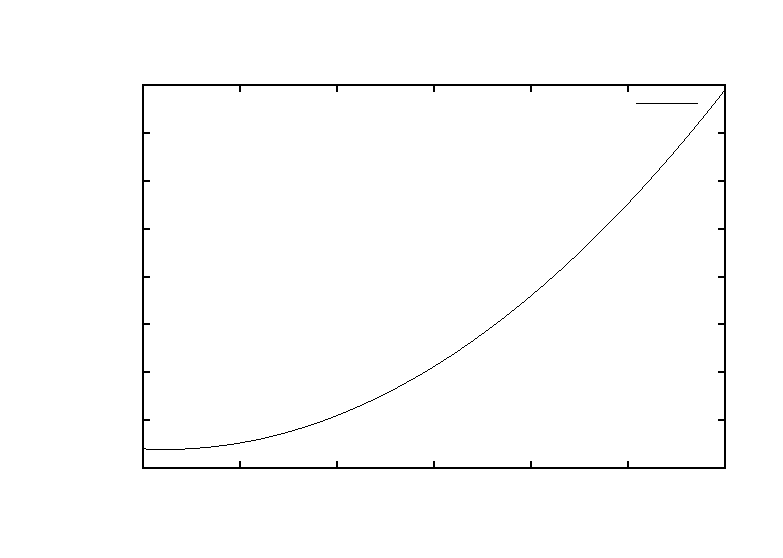
\includegraphics{plot}}%
    \gplfronttext
  \end{picture}%
\endgroup
}
  \caption{graph of slipstream correction factor.}
\end{figure}
\end{frame}

\begin{frame}
\frametitle{Physiological Model}

\begin{columns}
  \begin{column}{0.6\textwidth}
    \begin{itemize}
    \item Muscule stuff
    \end{itemize}
  \end{column}
  
  \begin{column}{0.4\textwidth}
    \begin{figure}[ht!]
      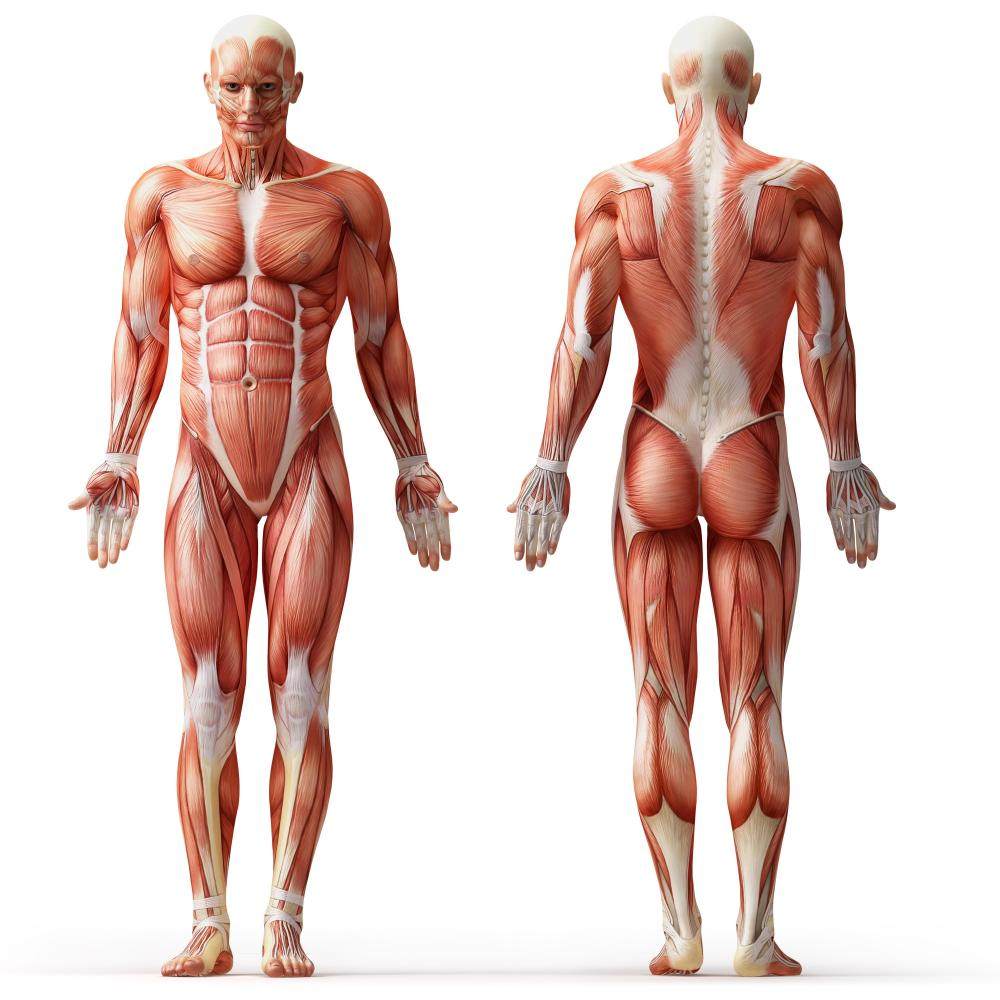
\includegraphics[scale=0.12]{physiological.jpg}
    \end{figure} 
  \end{column}
\end{columns}

\end{frame}

\begin{frame}
\frametitle{Psychological Model}

\begin{columns}
  \begin{column}{0.5\textwidth}
    \begin{itemize}
    \item Brain stuff
    \end{itemize}
  \end{column}
  
  \begin{column}{0.5\textwidth}
    \begin{figure}[ht!]
      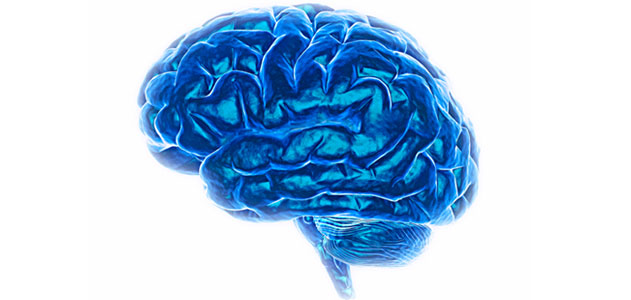
\includegraphics[scale=0.3]{psychological.jpg}
    \end{figure} 
  \end{column}
\end{columns}

\end{frame}


\begin{frame}
\frametitle{Step 2: Game Theory - Preliminaries}

\textbf{Pay-off matrix}\\
The pay-off each player gets by playing certain strategies is contained in a matrix, we call this the pay-off matrix. By using this matrix, players can choose the best strategy they should play in certain situations.

\begin{example}[Pay-off matrix]
\begin{table}[ht!]
	\hspace{-4em}
	\centering
	\begin{tabular}{ccccc|}
		& & \multicolumn{3}{c}{Player 2}                                \\ \cline{3-5}
		& & A & B & \multicolumn{1}{c}{C}                               \\ \cline{3-5}
		\multirow{3}{*}{Player 1} & \multicolumn{1}{|c|}{a} & (2,1) & (1,3) & (7,2) \\
		& \multicolumn{1}{|c|}{b} & (4,3) & (5,9) & (6,7)                           \\
		& \multicolumn{1}{|c|}{c} & (3,1) & (1,2) & (7,4)                           \\ \cline{3-5}
	\end{tabular}
\end{table}
\end{example}

\end{frame}

\begin{frame}
\frametitle{Step 2: Game Theory - Model}
\begin{block}{2-racer Escape Case}
	\begin{itemize}
		\item 2 players
		\item Cooperation strategy
		\item Fall back strategy
		\item Break away strategy
	\end{itemize}
\end{block}
\end{frame}

\begin{frame}
\frametitle{Step 2: Game Theory - Model}
\begin{block}{Repeated games}
	\begin{itemize}
		\item Pay-off matrices - one-off games
		\item Will specify our repeated game depending on moments $\delta^{(n)}$
	\end{itemize}
\end{block}
\end{frame}

\begin{frame}
\frametitle{Step 2: Game Theory - Model}
\begin{block}{Pay-off dependencies}
	\begin{itemize}
		\item Probability of finishing first depends on $CS_{i,n} = \dfrac{P_{ped_{i,n}} \cdot \delta^{(n)}}{E_{i,n} \cdot v},\ i\in\{1,2\}$
		\item Advantage from drafting: $F_{draft}(x) = (0.62 - 0.0104 d_w + 0.0452 d_w^2)\cdot (1/2)\cdot c_d\cdot \rho\cdot A\cdot x^2$ where $x$ is the speed of the player
		\item Future work
	\end{itemize}
\end{block}
\end{frame}

\begin{frame}
\frametitle{Step 2: Game Theory - Model}
\begin{block}{Both players cooperate}
	\begin{itemize}
		\item Players choose to help each other
		\item The advantage will tend to go to the player that is second
		\item Pay-off for the player who is second is: $(1-P)\cdot \dfrac{F_{draft}(s)}{F_{max}} + 1$
	\end{itemize}
\end{block}
\end{frame}

\begin{frame}
\frametitle{Achievements and Contribution}

\begin{itemize}
	\item Implemented the proposed simulation in papers %add details
	\item Combined psychological model with performance model
	\item Game theoretical model which could be valuable for simulating races
\end{itemize}

\end{frame}

\begin{frame}
\frametitle{Future work}
  \begin{itemize}
  \item{On the simulation}
    \begin{itemize}
    \item Tools for result analysis
    \item Wider diversity of strategies
    \item Better GUI
    \end{itemize}
    
    \pause
    
    \vspace{0.3cm}

  \item{On game theory}
    \begin{itemize}
    \item Try to find an analytic formula for the value of the game
    \item Integrate it with the simulation
    \end{itemize}
  \end{itemize}
\end{frame}

\begin{frame}
\frametitle{Recap}

\begin{itemize}
	\item TODO
\end{itemize}

\end{frame}


\begin{frame}
\frametitle{Thank you!}

\huge
\centering Q\&A

\end{frame}

% End of slides
\end{document} 
